\chapter{Case study}
\label{chapt:Case study}

In this chapter we go over what it is exactly we did in the case study.
We go over the requirements of the system and how that influenced the choice we made in the previous chapter on which model to implement and research.
Apart from the target system we also discuss the technology used and how we build up the different models, their architectures and where the big differences between the models can be found.

\section{Target system: BESC}
The target system for our case study  is the BESC application developed by 4DVision\footnote{\url{http://www.4dvision.be/}}. 
This is a system used for importing and exporting cargo in or out of Congo.
The system consists of exporters and forwarders which are associated with a company and which need to make a visa request for importing/exporting goods.
These visa requests then have to be approved by the agents assigned to that forwarder/exporter. 
These agents can approve only a certain number of requests depending on the visa points they have available, they can also request corrections on visa requests or refuse the visa requests.
In general agents are assigned to exporters and forwarders depending on the country from which they operate and their language.
Between agents there is a hierarchy with national/global/control agents that do supervision and provide additional visa points.
\\
\\
This system's access control is currently done by statically checking if given roles are allowed to access certain objects, putting the role checks in the code. 
With our models we provide a more dynamic approach to access control, this means that we can change the access control rules while the system is running.
An admin can then configure the different models depending on the needs, this means no new development is required when the access control needs change.
Apart from this requirement of dynamic access control the models should be able to meet following requirements that are in the original BESC system:
\\
\begin{enumerate}
    \item Objects can only be accessed if a rule has been made for the objects, if no rule exists nobody has access. Only those users conforming to the rule can access it. This includes rules saying everyone has access to that object.
    \item Only users that are logged in can be granted access, all others are denied by default.
    \item Get, Put, Post and delete should be supported.
    \item It should be possible to add custom actions that have access rights attached to them.
    \item It must be possible to only be able to access objects when one of their fields has a certain value.
    \item It must be possible to hide certain objects their fields if no access to that field is granted. The user should not even know the existence of the fields.
\end{enumerate}
\\
With the last two requirements it becomes clear that there is a need for fine grained access control where we can deny access depending on the values of certain fields (which will be our attributes) or deny access to these fields as a whole.
The role based access control model as described in the previous chapter does not allow for this kind of fine grained access control, meaning that another model has to be decided on.
Attribute based access control meets these requirements and this is due to the introduction of attributes.
Given these two observations we look for models that are a hybrid version of the two models.
We need a hybrid that combines the concepts of role based access control and introduces the concept off attributes and conditions from attribute based access control to allow for fine grained access.
We find these needs fulfilled using the attribute enhanced role based access control model, which is the model we use instead of the role based access control model.

\section{Approach}
There are two main options for adding access control models into this application.
The first option is to use existing frameworks that have already implemented these models, the second option is to implement these models into the BESC application ourselves.
Both these approaches have their positives and negatives which have to be taken into consideration before choosing which approach we take.
\\
\\
The positive points of the first option are that in this case we already have a working solution that is less likely to contain errors and a solution that has a tried and tested user interface adapted to the needs of using the models properly. 
The downsides however are that because attribute enhanced role based access control is rather novel there are no out of the box solutions for it yet, meaning we would have to create this ourselves.
For attribute based access control the implementations that are available are generally not open source and those that are are not mature enough yet.
This would also require us to learn how to setup the different systems and how they can be applied to the existing application that we test.
\\
\\
For option two the positives are that when implementing these models ourselves we can control the environment properly and implement the models in a similar way.
This to make sure that the differences and problems noticed are caused by the nature of the models and not because the solution provided for one model is better developed or uses better technology than the solutions that are available for the other model.
The downsides are that by developing this ourselves we are limited to what we can create ourselves, we wont be able to reach the quality of out of the box solutions with years of development that have a high quality user interfaces while we are working on this with limited time and resources.
Some scoping has to be done here which we have to take into account when doing the study,making sure that the metrics gathered and questions asked research what is in the scope of our study, we discuss this further in the next chapter. 
We are also required to go in depth into the architecture of the existing application in order to integrate our security models into it.
This also requires learning a new language and using a new environment since the original application has been build using C\# in the .net core framework, with which we have no prior experience.
\clearpage
We have chosen to go with option two, since there are no existing implementations yet for attribute enhanced role based access control that are available we have to provide this ourselves either way. 
Because of this we already have to overcome most downsides of approach two even if we were to choose an existing implementation of the attribute based model, this makes it logical to also implement the attribute based model ourselves.
Doing so ensures that the models have the same grounds of comparison, use the same technologies and have the same abilities if it comes to creating rules.
This also gives us optimal flexibility when we need to adapt the systems to our needs as stated in the requirements.

\section{Technology and implementation}
As mentioned before the BESC application is written in C\# and makes use of the .net core framework, we also implement our models using this language and framework.
Different components are needed, we divide the models in 3 different parts:
\begin{enumerate}
    \item The management component, this component is made for the management of users, their roles, adding permissions and attaching them to roles in the attribute enhanced role based model and adding policies for the attribute based model, including their conditions. 
    This allows for adding and removing each of these entities to the system (except users which is already available in BESC) and setting up the relationships between them.
    \item The access control component, this is the component that upon receiving a request for access gets all the policies/permissions involved and makes use of the evaluation component to determine if access is allowed. 
    This is the component that checks if the rules are positive or negative depending on the result of the evaluation of the conditions.
    It also keeps track of fields that have been hidden and takes the appropriate steps to make sure they do not get passed to the front of the application.
    It is also this component that is responsible to add the needed queries when partial access is allowed.
    \item The evaluation component, this component evaluates the different conditions put on the policies/permissions and checks if a condition is met or not, which is used by the access control component to make a decision on allowing access or not.
\end{enumerate}


\subsection{Management component}
In this section we go over the management component implemented in BESC, this for both models.

\subsubsection{Attribute enhanced role based access control}
The image below shows the database scheme of the structure of managing the system, this resembles most architectures used for role based access control:
\\
\begin{figure}[h]
    \centering
    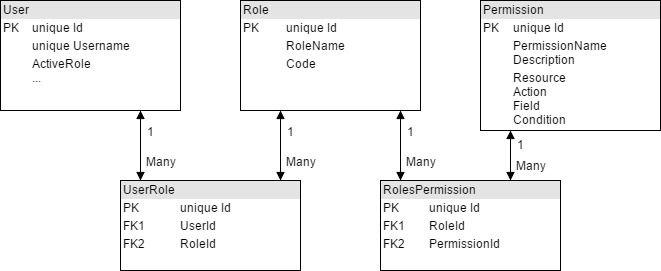
\includegraphics[width=0.7\textwidth]{Img/self/RBACManagementDiagram.jpg}
    \caption{Database diagram for AERBAC management}
\end{figure}
\\
We see that we have users with some fields, username Id etc but most importantly their active role. Since the system allows for users to have more roles and being able to switch between those roles we use this field to keep track of the user his current role.
Then we have the role objects in the system which have a code and name, all that is needed for a role to be identified in a system.
The third important part is the permission, it has multiple fields with the most important ones being Action, Resource, Condition and Field. 
The action represents what action can be done on the objects of type resource, possibly with a certain condition that allows viewing a specific field of that object.
These last two are optional.
Apart from these three we have some helper tables to allow for our many to many relationships where multiple users can be associated with multiple roles and multiple roles can be associated with multiple permissions.
The attribute enhanced aspect of the model is primarily contained in the Condition and Field attribute fields of the permissions.
\\
\\
Another part of the management component is the user interface, the user interface is used for the admin of the system to add new roles, assign these to users, add permissions and assign these to roles.
In our case study we have made a very basic user interface to allow these functions .
Below you can see how permissions are added to the system as well as how we add roles and assign them to users and assign permissions to roles.

\begin{figure}[h]
    \centering
    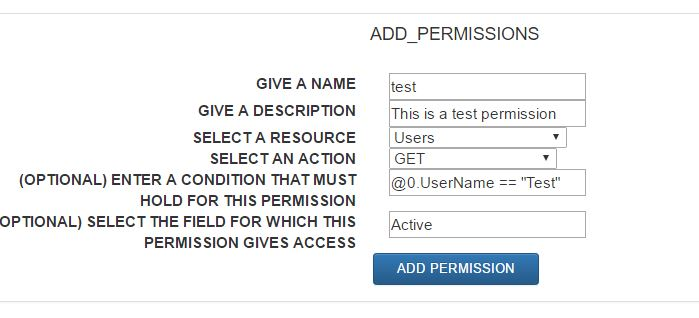
\includegraphics[width=0.7\textwidth, height=0.22\textwidth]{Img/Tool/AddPermission.JPG}
    \caption{Adding permissions in AERBAC}
\end{figure}
\begin{figure}[h]
    \centering
    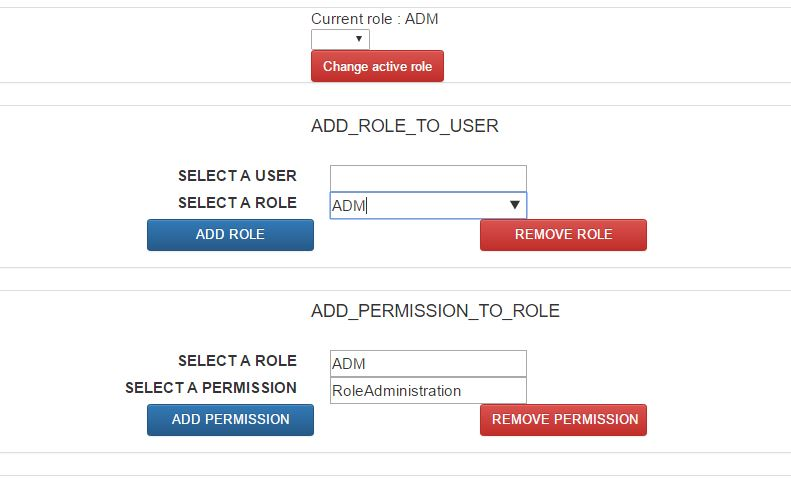
\includegraphics[width=0.8\textwidth, height=0.45\textwidth]{Img/Tool/RBAC_AddRP.JPG}
    \caption{Adding roles and permissions and changing roles in AERBAC}
\end{figure}

\subsubsection{Attribute based access control}
The image below (3.4) shows the database scheme of the structure of managing the system using the attribute based access control model:
\begin{figure}[h]
    \centering
    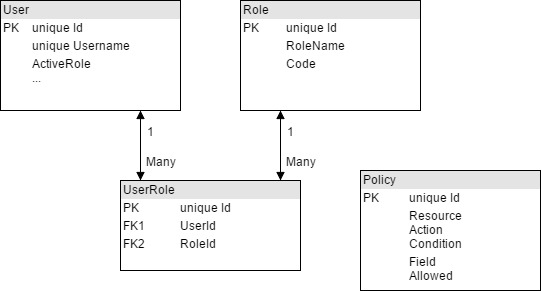
\includegraphics[width=0.7\textwidth]{Img/self/ABACManagementDiagram.jpg}
    \caption{Database diagram for ABAC management}
\end{figure}
\\
\\
Just like in the previous model we have users and roles, the only reason however that we have roles like this is because we want the system to support having multiple roles on a single user, this model could just as well do without the roles.
Unlike the previous model roles are not first class citizens here over the other objects and their attributes.
Once again we also have a helper table for the relationship between users and roles.
Instead of permissions however we now work with policies, these policies have no relationship with any of the other parts.
The important fields in these policies are Action, Resource, Condition, Field and Allowed. 
Again these mean practically the same as with the previous model, except that now a condition is not optional and should always be provided and the allowed field, which allows for setting both positive and negative policies.
The negative policies are stronger than the positive ones and if the condition on these negative policies is met then access is denied completely.
\\
\\
Once again a very basic user interface for the admin of the system, in the attribute based model the admin can add roles, assign users to roles and add policies to the system.
The interface is specifically kept as close as possible to the previous one in order to try and minimize the effects of the user interface on using both models.
Below you can see how policies are added to the system as well as how the UI looks like for adding roles and assigning them to users and for users to change their active roles.

\begin{figure}[h]
    \centering
    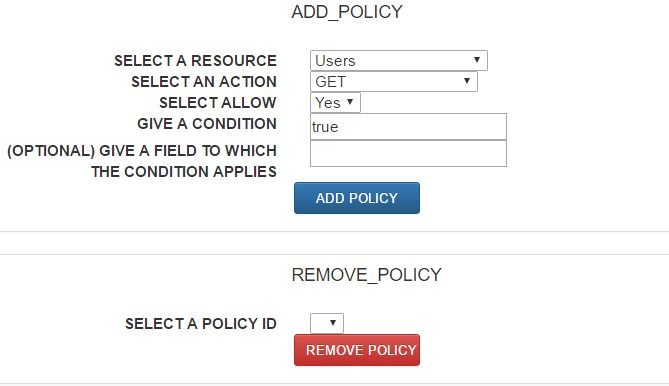
\includegraphics[width=0.7\textwidth]{Img/Tool/AddPolicies.JPG}
    \caption{Adding policies in ABAC}
\end{figure}
\clearpage
\begin{figure}[h]
    \centering
    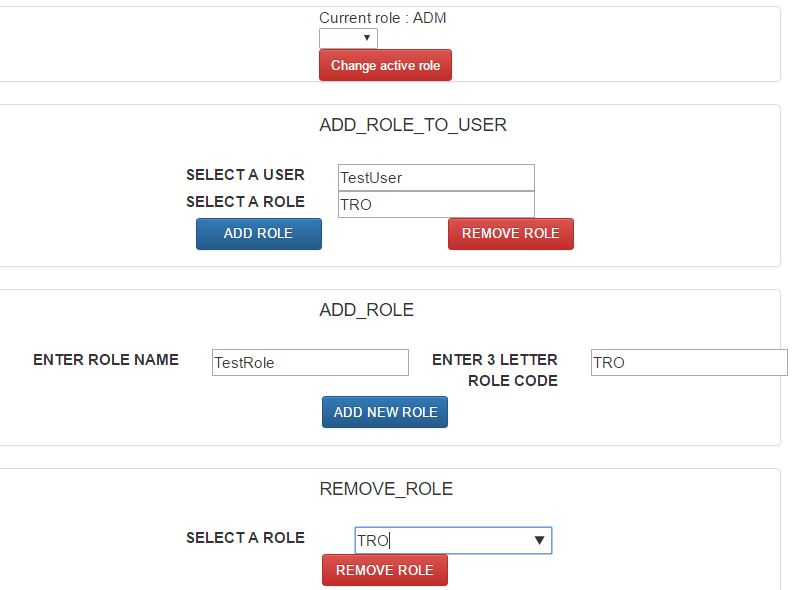
\includegraphics[width=0.7\textwidth]{Img/Tool/ABACADD.JPG}
    \caption{Adding and assigning roles in ABAC}
\end{figure}

\subsection{Access control component}

We implemented the  access control component in 2 layers, first we have a layer that checks if a user can do the requested action on the type of object, without looking at values of the attributes of the different objects.
Doing this prevents  that we already have to access the objects and do conditional checks if we are not supposed to access those objects at all, independent of the values of the attributes.
This is to prevent unnecessary computations taking up extra time.
The second layer is when conditions have to be applied to specific objects and the user can only do something with a subset of that object type.

\subsubsection{Attribute enhanced role based access control}
In the case of attribute enhanced role based access control we have 3 different cases:
\begin{itemize}
    \item There is no condition on the permission at all.
    \item The conditions only contain attributes that are not part of the object we want to access, such as user data.
    \item The conditions contains attributes of the object we want access to.
\end{itemize}
\\
In case one and two we can do the evaluation in layer one, we do not need specific object data to evaluate these conditions.
In case three we already need to be able to access the object before the condition can be evaluate, if there was already a negative response in the previous layer this will not be executed.
When using the fields option, which allows for hiding certain attributes from the users, the permission only counts for the field in question on that object, not general access to the object.
Once such a permission is made the field is invisible for everyone who does not meet this permissions condition.
This functionality is also part of the second layer.


\subsubsection{Attribute based access control}
In the case of attribute based access control we have only 2 cases since we must always have a condition on the policies:
\begin{itemize}
    \item The conditions only contain attributes that are not part of the object we want to access, such as user data, this includes conditions that just contain true.
    \item The conditions contains attributes of the object we want access to.
\end{itemize}
\\
Analogous to the previous model we have that the first case is checked in the first layer, the second case is checked in the second layer if we get there.
\\
\\
When using the fields option, which allows for hiding certain attributes on the objects from the users, when a policy is set for hiding a field then everyone who does not meet the policy cannot see the field.
This policy however only affects the fields, it does not deny or grant access to the object as a whole another policy has to be made for that.
Again this functionality is also a part of the second layer.
\\
\\
Another specificity with the attribute based model is that we have the option of negative policies.
The negative policies are always evaluated first and are the strongest policies, if the condition of a negative policy is met this means there is no access allowed at all.

\subsection{Evaluation component}
This component is a component that is used in both models in the same way.
Building this component mainly relies on the use of the dynamic LINQ library\footnote{\url{https://github.com/StefH/System.Linq.Dynamic.Core}}.
This is an extension to the linq (language integrated query) functionality that is part of the .net framework, this lets us use a query syntax in the code, which allows queries to be generated from code with similar syntax.
Dynamic linq allows to apply the query capabilities linq provides by using and evaluating strings while the system is running.
Depending on the difficulty of the queries this is evaluated either on database level or on code level (or both).
Doing this allows for a language that the participants in our study are familiar with since it resembles the capabilities of the programming language they are used to.
\\
Below is an example of the conditions we have, this is for the attribute based model:
\begin{algorithm}
    (Code == "FWD") and @0.ActiveRole == "ADM"
\end{algorithm}
\\
This is a piece of code to access the roles that are available in the system, this condition checks if the Code field of the role object we want to access has the value "FWD" and if the current user has as its active role "ADM".
We can see a few different features of using dynamic linq here that make it useful for using as the core part of our evaluation component:
\begin{itemize}
    \item Access to the fields of the object you are working on just by using their field names (the Role object has a field Code). The fields can also be chained just like while programming to get objects that can be part of that object using the . operator.
    \item Availability of boolean operators and, or, not as well as the use of ( and ) to form boolean expressions.
    \item Can input constant strings with "" and other constants just as in normal programming.
    \item Availability of placeholders that can be put into the conditions that can make use of attributes of other objects if needed. This is generally done to get external attributes into the system. In the example we can see this is done by using @ and then the number of the object that is available. In the case of the example we have @0 which is where the object of the user making the request is contained and then the field of that object, its ActiveRole.
\end{itemize}
